\documentclass[11pt,a4paper]{article}
\usepackage[margin=23mm]{geometry}
\usepackage{fontspec,amsmath,amssymb,booktabs,graphicx,xcolor,hyperref,fancyhdr}
\setmainfont{DejaVu Sans}
\definecolor{ink}{HTML}{163746}
\definecolor{accent}{HTML}{3F6E63}
\hypersetup{colorlinks=true,urlcolor=accent,linkcolor=ink,pdftitle={MILPA-360: fundamentos y decisiones V4}}
\pagestyle{fancy}\fancyhf{}\fancyhead[L]{\small MILPA-360 / BioMars Chiapas}\fancyhead[R]{\small V4 · 21 sep 2026}\fancyfoot[L]{\scriptsize Concepto y cálculo; sin validación física}\fancyfoot[R]{\thepage}
\setlength{\headheight}{15pt}\emergencystretch=2em\setlength{\parindent}{0pt}\setlength{\parskip}{7pt}
\input{valores.tex}
\begin{document}
{\Huge\color{ink} Un sistema visible.\\Una propuesta trazable.}\par
{\large Fundamentos físicos, químicos, matemáticos y visuales de MILPA-360}

\textbf{Responsable:} Aldo Fabio Contreras Marroquín · BioMars Chiapas.

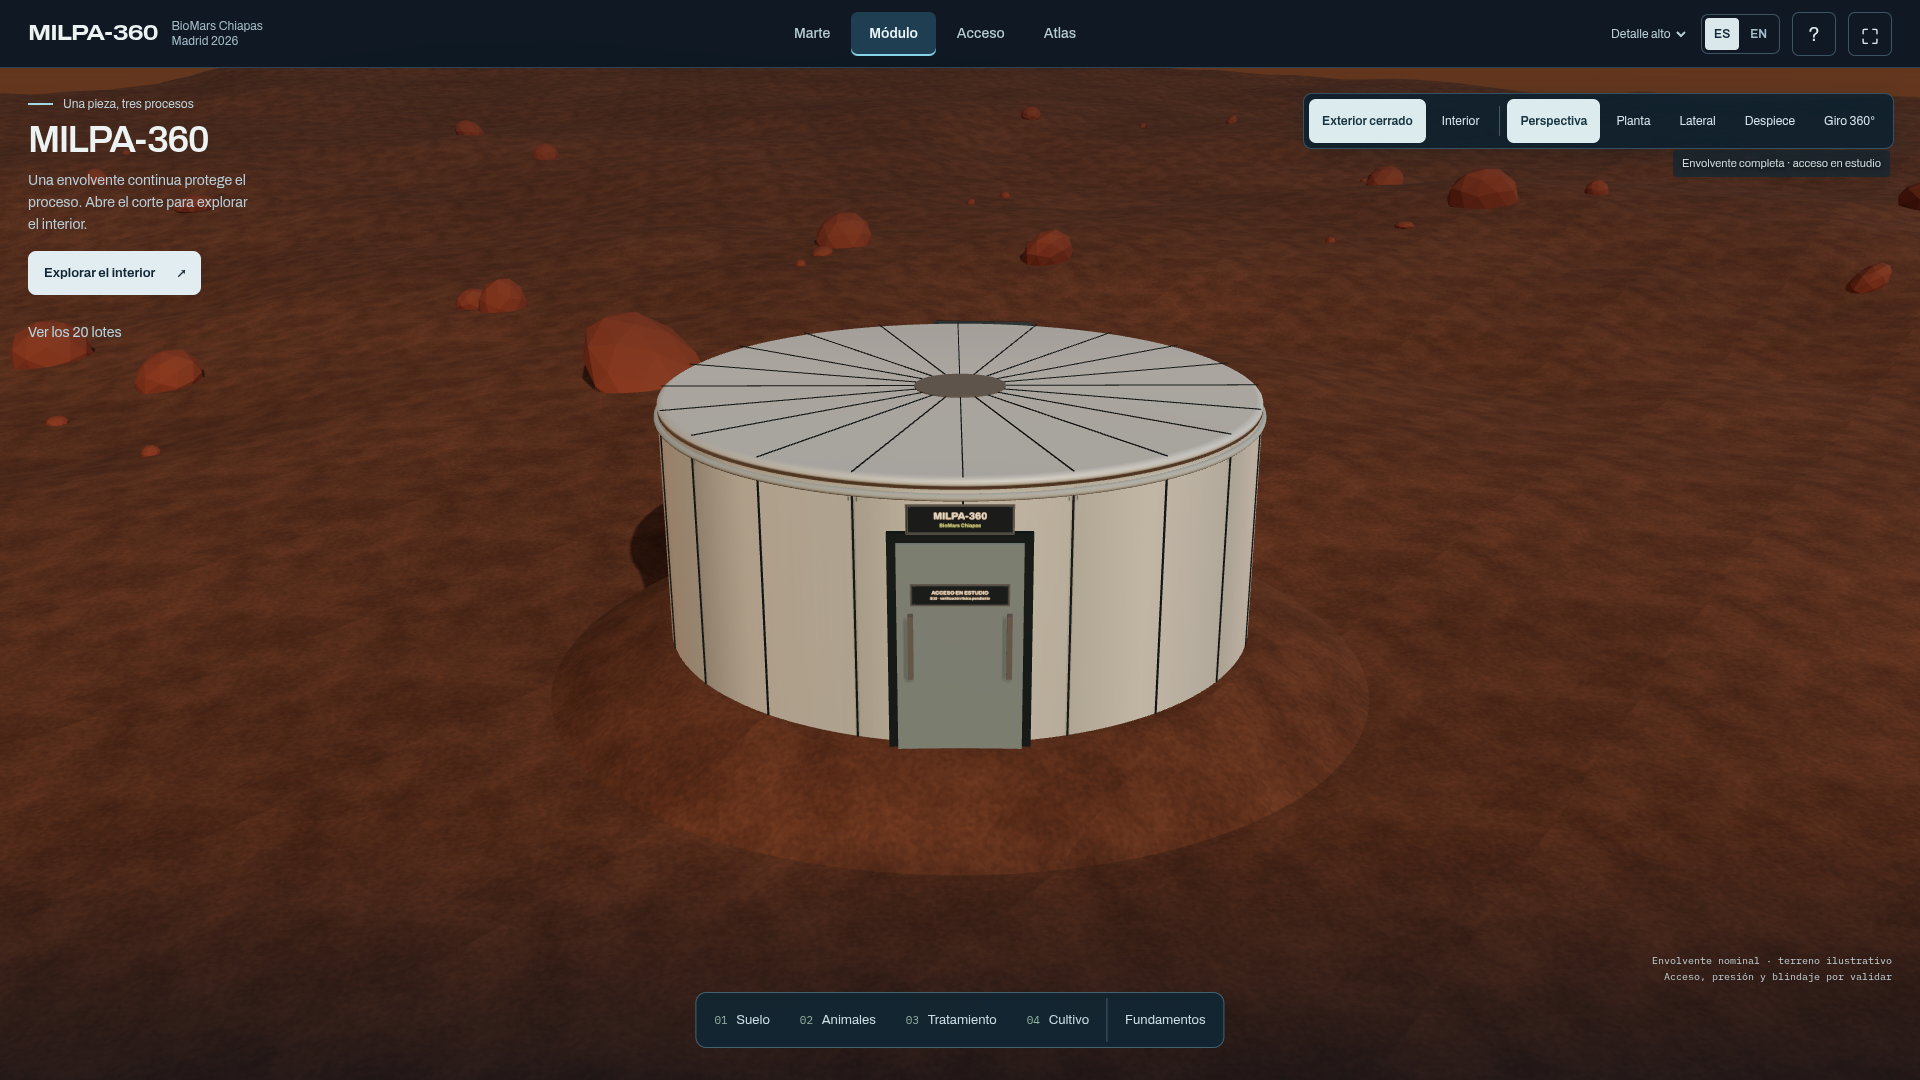
\includegraphics[width=\linewidth]{../../../docs/madrid/capturas-v4/exterior-es.png}

\textbf{Qué se cierra aquí.} Una revisión digital reproducible: geometría nominal,
modelo por lotes, exterior cerrado, inspección, simulación ilustrativa, documentos y
paquete sin Internet. La imagen representa una envolvente de integración; no es un
recipiente a presión aprobado ni prueba de que el acceso B19 sea seguro.

\textbf{Cómo leer las cifras.} Un valor puede ser requisito, literatura, hipótesis,
cálculo o medición. En esta memoria no se inventan mediciones. Las fórmulas siguientes
explican los resultados de los scripts existentes y sus límites de aplicación.

\textbf{Reproducción.} Desde la raíz: \texttt{python3 analysis/fundamentos\_latex.py}.
El archivo de parámetros, cálculos y geometría es la fuente de las macros numéricas.
Las fuentes LaTeX están en \texttt{docs/madrid/latex/}.\\
El PDF y los valores generados quedan en \texttt{outputs/madrid-s5/}. Tectonic 0.17.0 compila el documento.

\newpage
\section*{1. Geometría, superficie y masa}
Un sector de anillo entre $r_i$ y $r_o$, con ángulo $\theta$ en radianes, tiene área
\begin{equation}
 A=\int_0^\theta\int_{r_i}^{r_o}r\,dr\,d\varphi
 =\frac{\theta}{2}(r_o^2-r_i^2).
\end{equation}
Para $N=20$ posiciones, el paso es $\Delta\theta=2\pi/N=18^\circ$.
La geometría deja un 6\% de separación angular: $\theta=0.94\,\Delta\theta$.
El reborde digital $b=0.035\,\mathrm{m}$ se descuenta mediante la construcción
\begin{align}
 r_i'&=r_i+b, &r_o'&=r_o-b, &\theta'&=\theta-\frac{2b}{(r_i+r_o)/2},\\
 A_u&=\tfrac12\theta'({r_o'}^2-{r_i'}^2).
\end{align}
La reducción angular es la definición adoptada por el generador, no una afirmación
sobre la tolerancia de una pieza fabricada. Con $r_i=1.58\,\mathrm m$ y
$r_o=2.18\,\mathrm m$, $A_u=\AreaCartucho\,\mathrm{m^2}$ por cartucho.
\begin{center}\begin{tabular}{ll}\toprule
Magnitud nominal & Resultado\\\midrule
Diámetro y altura del casco & $4.56\,\mathrm m$ y $2.20\,\mathrm m$\\
Superficie de los 20 cartuchos & $\AreaTotal\,\mathrm{m^2}$\\
Superficie de los 12 cartuchos de cultivo & $\AreaCultivo\,\mathrm{m^2}$\\
Profundidad de sustrato & $0.22\,\mathrm m$\\
Masa nominal de sustrato por cartucho & $\MasaCartucho\,\mathrm{kg}$\\\bottomrule
\end{tabular}\end{center}
El volumen de sustrato y su masa se calculan como
\begin{equation} V_s=N A_u h,\qquad m_s=\rho V_s.\end{equation}
Con $\rho=1500\,\mathrm{kg/m^3}$ supuesto, la masa total de sustrato es
aproximadamente $1697\,\mathrm{kg}$. Cambiar de gravedad reduce $W=mg$, no la masa,
la inercia o la energía para tratar el material. Densidad operativa, humedad y tara
requieren pesaje; no se suman masas seca y húmeda sin definir su base.

\textbf{Hallazgo geométrico.} La huella circular de $16.33\,\mathrm{m^2}$ no es superficie
cultivada. El área de cultivo es $\AreaCultivo\,\mathrm{m^2}$, porque existen pasillo,
equipos, regeneración, rebordes y separaciones. Este denominador evita sobreestimar
el alimento. Fuente reproducible: \texttt{analysis/milpa360\_p2.py}.

\newpage
\section*{2. Luz, energía y térmica}
La integral diaria de luz y el consumo de una luminaria idealizada son
\begin{align}
 \mathrm{DLI}&=\frac{\mathrm{PPFD}\ t_h\ 3600}{10^6}
 &&[\mathrm{mol\,m^{-2}\,d^{-1}}],\\
 P_{\mathrm{LED}}&=\frac{\mathrm{PPFD}\ A_c}{\eta_{\mathrm{LED}}}
 &&[\mathrm W],\\
 E_{\mathrm{LED}}&=\frac{P_{\mathrm{LED}}\,t_h}{1000}
 &&[\mathrm{kWh/d}].
\end{align}
$\mathrm{PPFD}$ se expresa en $\mu\mathrm{mol\,m^{-2}\,s^{-1}}$ y
$\eta_{\mathrm{LED}}$ en $\mu\mathrm{mol/J}$. El cálculo presupone luz útil sobre el
área declarada; distribución espacial, pérdidas ópticas y sombreo necesitan medición.
La suma por especies da $\LuzNominal\,\mathrm{kWh/d}$ con los supuestos vigentes.

La energía química del metano no equivale a electricidad:
\begin{equation}
 E_{\mathrm{quim}}=\frac{V_{\mathrm{gas}}x_{\mathrm{CH_4}}\,\mathrm{PCI}_{\mathrm{CH_4}}}{3.6},
 \quad E_{\mathrm{el,neta}}=\eta_{\mathrm{el}}E_{\mathrm{quim}}-E_{\mathrm{aux}}.
\end{equation}
Con volumen en $\mathrm{m^3/d}$ y PCI en $\mathrm{MJ/m^3}$, se obtienen
$\mathrm{kWh/d}$. Presión, temperatura, base seca/húmeda y sólidos volátiles deben
ser compatibles con la fuente del rendimiento. El caso nominal del proyecto produce
aproximadamente $\BiogasNominal\,\mathrm{kWh/d}$ químicos; para provisiones se adopta crédito
eléctrico cero hasta seleccionar conversión y auxiliares.

La transmisión térmica estacionaria preliminar es
\begin{equation}
 \dot Q=UA(T_i-T_e),\quad A=2\pi RH+2\pi R^2,
 \quad E_{24h}=\frac{24\dot Q}{1000}.
\end{equation}
No basta conocer la temperatura de Marte: $U$, puentes térmicos, radiación solar,
infiltración, metabolismo, evaporación y condensación afectan la carga. El escenario
nominal contabilizado arroja $\EnergiaNominal\,\mathrm{kWh/d}$ eléctricos, equivalente
a $\EnergiaSol\,\mathrm{kWh/sol}$. No dimensiona por sí solo un HVAC o soporte vital.

\textbf{Hallazgo de escala.} La luz nominal exige unas \RelacionLuz\ veces la energía química
nominal del biogás; incluso una conversión imposible del 100\% no cerraría esa demanda.
La diferencia justifica electricidad externa y una defensa como alimento complementario.
Fuentes: \texttt{milpa360\_p1.py}, \texttt{cierre\_acumulado.py}, BVAD/NASA y las
condiciones registradas en \texttt{registro-afirmaciones.csv}.

\newpage
\section*{3. Agua, residuos y química}
Para cada especie química o flujo material, la frontera del módulo exige
\begin{equation}
 \frac{dM}{dt}=\sum\dot m_{\mathrm{entrada}}-\sum\dot m_{\mathrm{salida}}+\dot m_{\mathrm{generación}}-\dot m_{\mathrm{consumo}}.
\end{equation}
Para masa total, generación y consumo se cancelan si se incluyen todas las especies.
Para un compuesto individual pueden existir reacciones. Larvas y digestor no pueden
recibir cada uno el 100\% de un mismo kilogramo inicial sin seguir las salidas intermedias.

En el modelo simplificado de cultivo, la reposición debida a evapotranspiración es
\begin{equation}
 W_{\mathrm{nuevo}}=(1-f_{\mathrm{rec}})W_{\mathrm{ET}},\qquad
 \tau=\frac{W_{\mathrm{inventario}}}{W_{\mathrm{nuevo}}}.
\end{equation}
Se calculan $6.302\,\mathrm{L/d}$ de ET y $1.260\,\mathrm{L/d}$ de reposición al suponer
80\% de recuperación. Con $40\,\mathrm L$, $\tau\approx31.7$ días sólo para esta frontera;
sin condensador son $6.35$ días. Agua humana, animal, limpieza, purgas y acceso de la
bomba quedan fuera: no se declara autonomía de todo el hábitat ni potabilidad.

La semirreacción de reducción completa del perclorato es
\begin{equation}
 \mathrm{ClO_4^-}+8\mathrm{H^+}+8e^-\longrightarrow\mathrm{Cl^-}+4\mathrm{H_2O}.
\end{equation}
Conserva Cl y O; carga izquierda $-1+8-8=-1$, igual a la derecha. El cloruro permanece
en el circuito hasta retirarlo: no desaparecen las sales. Para $M(\mathrm{ClO_4^-})
\simeq99.45\,\mathrm{g/mol}$,
\begin{align}
 m_{\mathrm{Cl^-}}&=m_{\mathrm{ClO_4^-}}\frac{35.45}{99.45},\\
 m_{\mathrm{DQO,ideal}}&=m_{\mathrm{ClO_4^-}}\frac{64}{99.45}.
\end{align}
Los 64 g corresponden al equivalente de dos moles de $\mathrm{O_2}$, ocho electrones.
No son una dosificación: biomasa, aceptores competidores, salinidad e inhibición
requieren ensayos. Lavar mueve el contaminante al agua; no lo destruye.

\textbf{Decisión sanitaria.} Salmuera y metanogénesis permanecen separadas. Sin método,
umbral, incertidumbre y análisis aceptable, el lote no se libera. Musgo y MFC no son
certificados de ausencia de perclorato o patógenos. Fuente: P1 y cierre acumulado.

\newpage
\section*{4. Movimiento, acceso y simulación}
La representación usa un anillo de veinte cartuchos; la posición lógica del lote es
\begin{equation}
 p_i(k)=(i+k)\bmod N,\qquad \theta_k=-\frac{2\pi k}{N}.
\end{equation}
La masa conserva identidad al cambiar de estación. El indexado nominal ocurre cada
ocho soles; su duración mecánica no está validada. El cambio suave visible usa
\begin{equation}
 x_{n+1}=x_n+(x_{\mathrm{objetivo}}-x_n)(1-e^{-\lambda\Delta t}).
\end{equation}
Se obtiene de $\dot x=\lambda(x_{\mathrm{objetivo}}-x)$ con objetivo constante. Por eso
la respuesta depende de tiempo, no de cuántos fotogramas tenga el ordenador.
$\lambda=9\,\mathrm{s^{-1}}$ es una elección visual; no una velocidad biológica ni el
perfil de un motor. El paso visual se limita a 50 ms para evitar saltos tras un bloqueo;
por debajo de 20 FPS la animación puede ralentizarse. El reloj visual se acumula sólo en reproducción: pausar no reinicia
las poses de las aves. El modelo de inventarios mantiene su paso fijo y su validación.

El dimensionado mecánico requiere, como mínimo,
\begin{equation}
 I\approx\tfrac12m(r_i^2+r_o^2),\quad
 \tau_{\mathrm{motor}}\geq I\alpha+\tau_{\mathrm{resistencia}},\quad P=\tau\omega.
\end{equation}
Rozamiento, arranque, guiado, freno y factor de diseño dependen de componentes reales.
La selección no se deduce de una malla o de un motor de maqueta a escala.

Al retirar $n$ posiciones, una cota geométrica del hueco interior es
\begin{equation}c(n)=2r_i\sin\!\left(\frac{n\pi}{N}\right).
\end{equation}
Con dos posiciones resulta $0.976\,\mathrm m$ antes de herrajes. No equivale al ancho
útil para una persona con herramientas ni para rescate. El estudio B19 conserva
retención y salida con pérdida de energía como requisitos; faltan aceptación física
y revisión ergonómica. NASA-STD-3001 Vol.2, requisitos 8013, 8014 y 8020, trata rutas,
tareas y emergencias; citarlo no certifica esta disposición.

\textbf{Presión y cubierta.} Para una pared cilíndrica delgada ideal,
$\sigma_\theta\approx\Delta pR/t$. Faltan $\Delta p$, material, juntas y espesor resistente:
no se calcula una resistencia ficticia. Los paneles, juntas y techo V4 son una
representación continua de integración, no un diseño de fabricación.

\newpage
\section*{5. Decisiones visuales y límites de cierre}
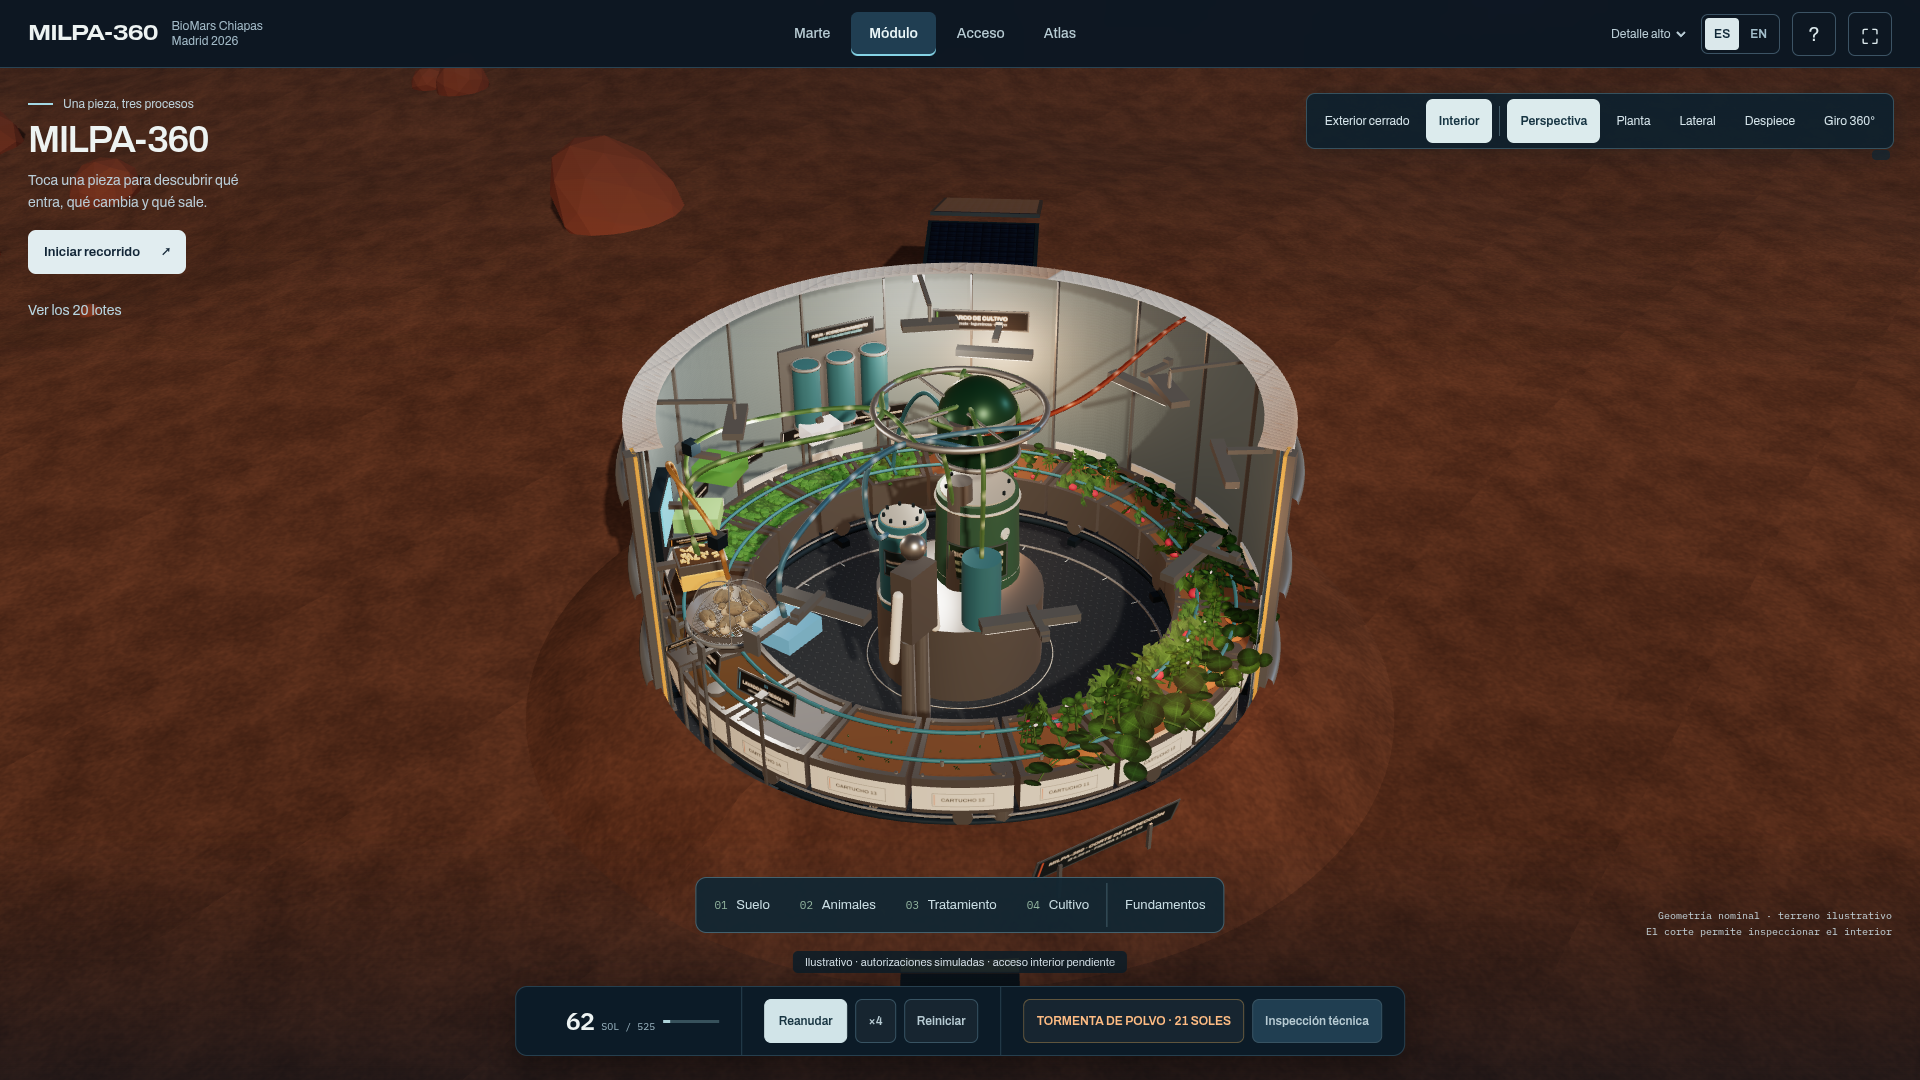
\includegraphics[width=\linewidth]{../../../docs/madrid/capturas-v4/interior-es.png}

\textbf{V4 implementada.} Exterior de 360 grados y techo derivado del casco; talud
continuo apoyado; conexión eléctrica visible; modos exterior/interior; navegación
por proceso; fórmulas locales MathML; selección directa y ES/EN. El corte es una
herramienta de inspección, no una abertura operativa. B19 conserva su visor separado.

\textbf{Rendimiento.} Los objetos internos se ocultan al cerrar la envolvente. Plantas
y musgo inactivos se excluyen del dibujo; el panel de datos se actualiza a 8.3 Hz.
La calidad automática ajusta resolución entre 0.65 y 1.25 píxeles de render por píxel
CSS, con decisiones cada tres segundos. La geometría y el modelo no cambian.
Mediciones reales, hardware y condiciones están en \texttt{PRUEBA-VISUAL-V4.json}.

\textbf{Escena y evidencia.} El mapa global Viking es NASA/JPL-Caltech, procesado por
USGS; el terreno y las estrellas son ilustrativos. No se inventa topografía local.
Las aves son figuras visuales y los soportes no acreditan cargas, capacidad sanitaria
ni funcionamiento marciano. No se presenta un render como fotografía experimental.

\textbf{Pendientes que no resuelve una búsqueda.} Autorización de delegación/formato,
feedback real, cotizaciones específicas, recursos disponibles, ensayos físicos,
análisis sanitario, proyector y aceptación mecánica necesitan evidencia externa.
La entrega digital conserva cada responsable y dato faltante en el cierre acumulado.

\textbf{Fuentes y lectura adicional.}
\begin{itemize}
\item \href{https://www.nasa.gov/reference/8-0-architecture-vol-2/}{NASA, Architecture, Vol.2}: acceso y tareas; consulta 21 sep 2026.
\item \href{https://threejs.org/docs/pages/InstancedMesh.html}{Three.js, InstancedMesh}: reducción de llamadas de dibujo; API local fijada en r160.
\item \href{https://tectonic-typesetting.github.io/en-US/install.html}{Tectonic}: compilador de esta memoria, 0.17.0.
\item \href{https://thegrandjam2026.mars-challenge.com/en/la-experiencia/como-funciona}{The Grand Jam}: final Getafe, 3--5 nov 2026; no acredita condiciones particulares del equipo.
\end{itemize}
\end{document}
